\chapter{Introduction à la physique des réacteurs}
\section{Du processus de fission au caractéristiques d'un réacteur}
\subsection{Carburant nucléaire}
\subsubsection{Énergie produite par fission nucléaire}

	\begin{wrapfigure}[12]{l}{5cm}
	\vspace{-5mm}
	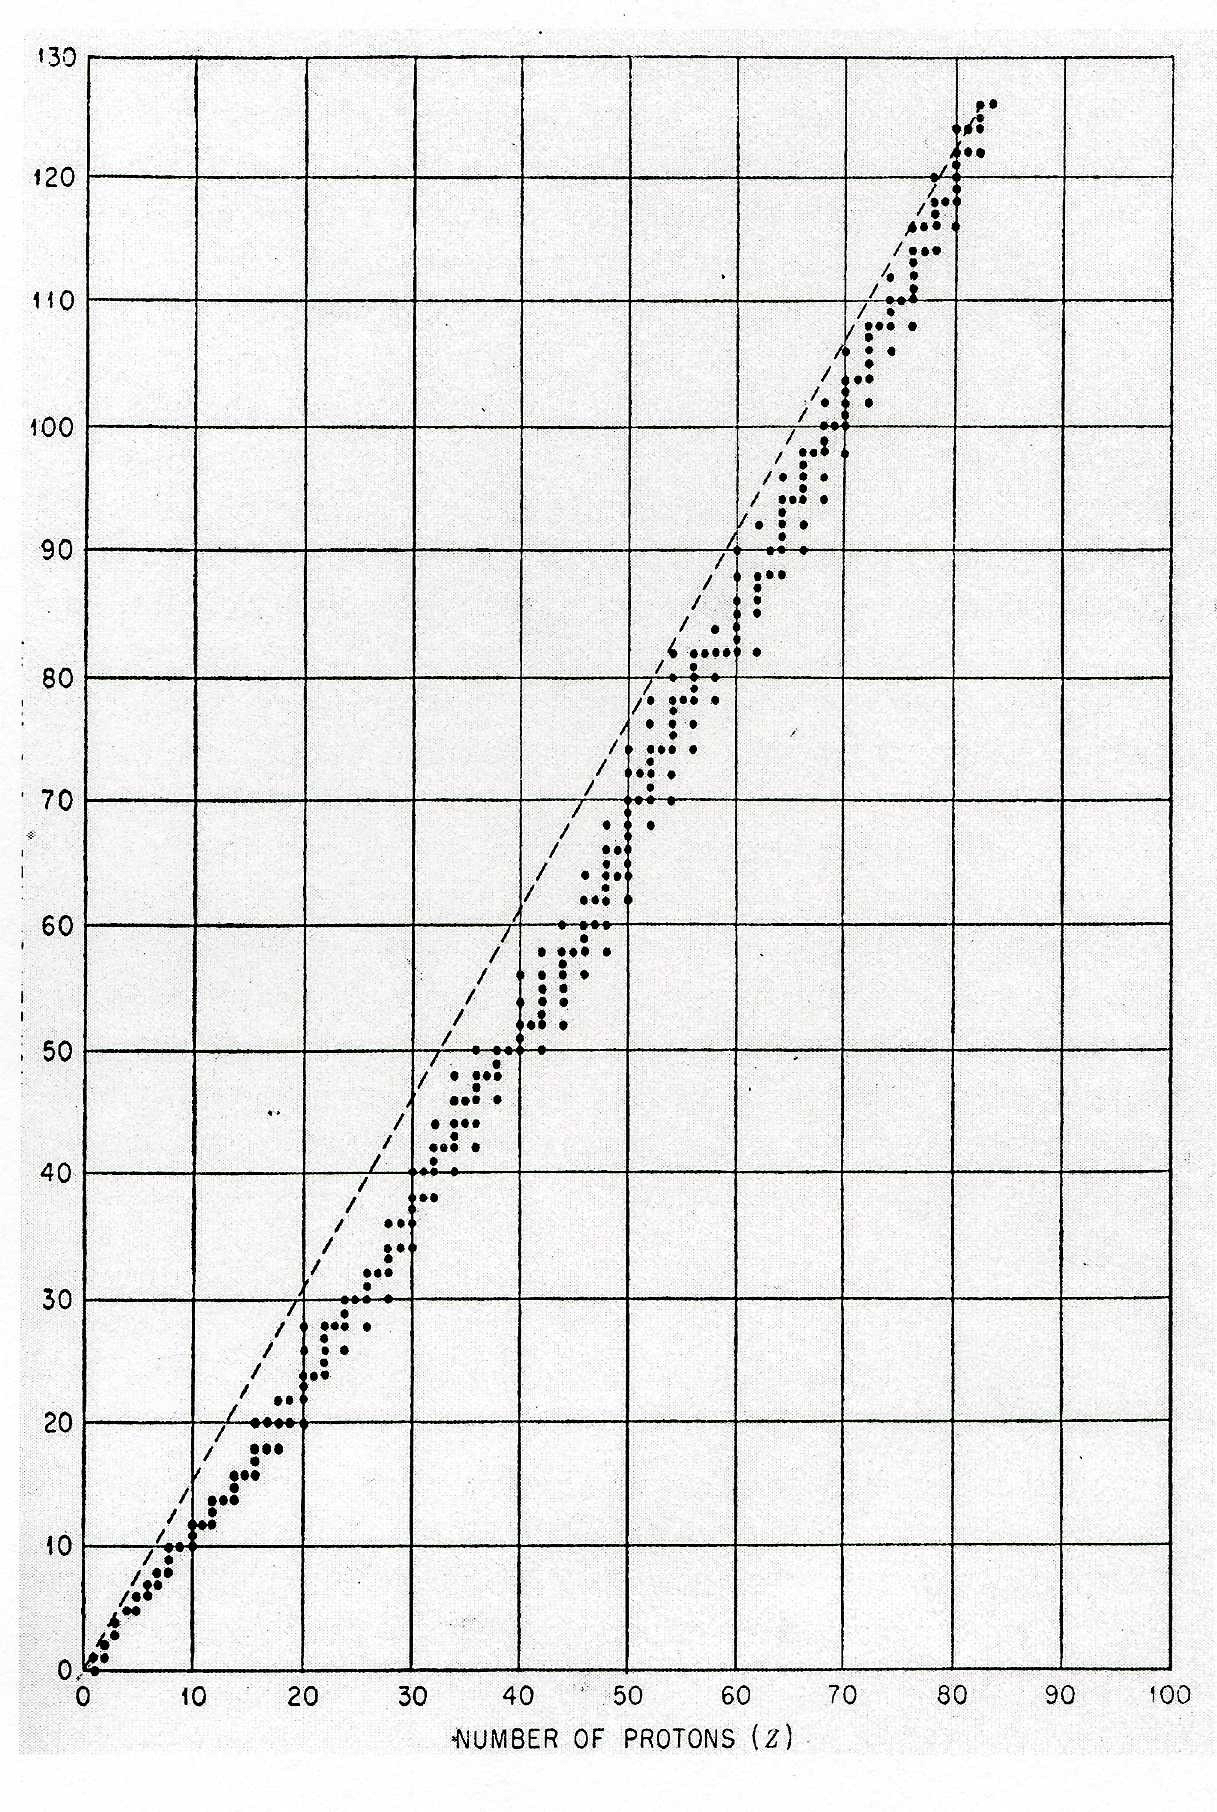
\includegraphics[scale=0.1]{ch1/image1.png}
	\captionof{figure}{ }
	\end{wrapfigure}
La stabilité des noyaux lourd est assurée par un excès du nombre de neutrons par rapport au 
nombre de protons. Le dernier élément stable est l'uranium $U$ ($Z=92$) que l'on trouve 
principalement en deux isotopes
\begin{enumerate}
\item $ ^{238}U$ $\approx$ 99.3\%
\item $ ^{235}U$ $\approx$ 0.7\%
\item $ ^{234}U$ $\approx$ traces
\end{enumerate}

Il existe une autre notation pour différencier les différents isotopes : elle consiste à écrire le symbole
de l'élément avec en indice le chiffre des unités du numéro atomique suivi du chiffre des unités du nombre
masse. Par exemple, on peut désigner $ ^{238}U$ par $U_{28}$ car dans ce cas Z = 92 et A = 238.\\

Lorsque l'on observe la valée de la stabilité, on peut en effet voir que plus le nombre de 
proton augmente, plus le nombre de neutron fait de même pour stabiliser le noyau. Si un 
noyau doit se fissionner, il y aura un trop pleins de neutrons et ces derniers peuvent 
être réutiliser à certaines fins.\\ 
\\


	\begin{wrapfigure}[8]{r}{3.4cm}
	\vspace{-8mm}
	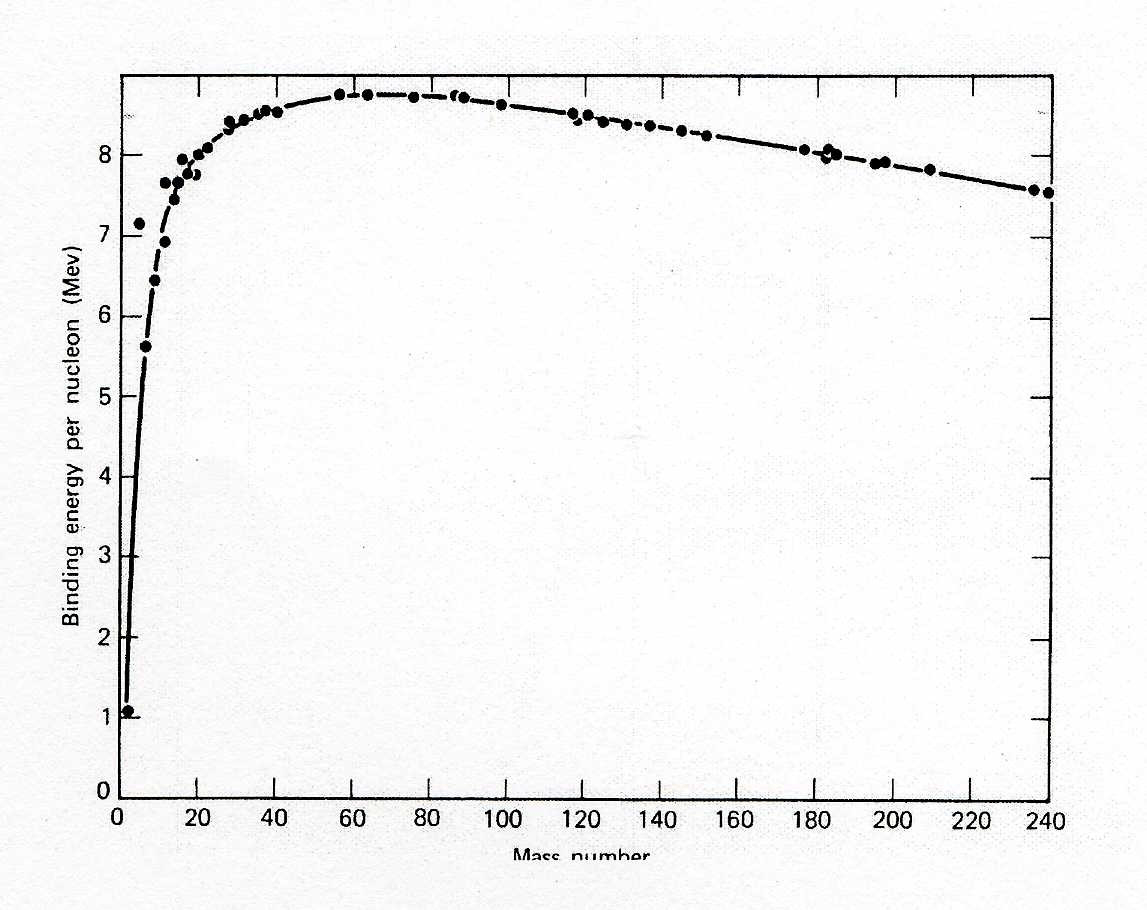
\includegraphics[scale=0.1]{ch1/image2.png}
	\captionof{figure}{ }
	\end{wrapfigure}
Une autre courbe connue est celle de l'\textit{énergie de liaison des noyaux}. 
On dit que les noyaux ont un défaut de masse car la somme des masses des nucléons
qui les constituent est plus élevée que la masse du noyau.
Cela implique qu'il existe une énergie de liaison dans le noyau afin que l'énergie
totale du système soit conservée. Cette courbe exprime cette quantité d'énergie
de liaison en fonction du nombre de masse des noyaux.\\

\begin{equation}
m_{noyau} c^2 < \Sigma_{nucléons} m_i c^2 \rightarrow E_{masse, noyau} + E_{liaison} = \Sigma_{nucléons} E_{masse}
\end{equation}

On remarque que les noyaux ont tendance à maximiser leur énergie de liaison 
\footnote{Pourquoi ?} et donc à
vouloir atteindre le sommêt de cette courbe qui se trouve aux alentours de A = 50.
Il est possible de récupérer pour d'autres fins l'énergie de liaison au moyen de réactions nucléaires, soit
en fissionnant des atomes lourds avec A > 50, soit en fusionnant des atomes légers avec A < 50.

\subsubsection{Isotopes fissiles et fertiles}
Les réacteurs nucléaires permettent de récupére l'énergie provenant du défaut de masse en fissionant des
noyaux. Pour cela, on bombarde des noyaux avec des neutrons, provoquant des fissions qui vont libérer
de nouveaux neutrons, donnant lieu à de nouvelles collisions pour arriver à une réaction en chaîne
auto-entretenue.\\

Parmi les éléments exploitables dans les réacteurs, il en existe qui vont directement libérer l'énergie
du défaut de masse. Ces isotopes sont qualifiés de \textbf{fissiles}. $U_{235}$ (naturel), 
$U_{233}, Pu_{235}$ par exemple sont des isotopes fissiles.

D'autres ne sont pas fissiles mais peuvent engendrer des isotopes fissiles par capture neutronique.
Ces isotopes sont qualifiés de \textbf{fertiles}.

\begin{equation}
\begin{array}{llll}
U_{238} + n\quad&\to\quad U_{239}+\gamma\quad&\overset{\underset{\Longrightarrow}{\text{23'}}}{\beta^-}\quad Np_{239}\quad&\overset{\underset{\Longrightarrow}{\text{2.3j}}}{\beta^-}\quad Pu_{239}
\vspace{2mm}\\
Th_{232} + n\quad&\to\quad Th_{233}+\gamma\quad&\overset{\underset{\Longrightarrow}{\text{22'}}}{\beta^-}\quad Pa_{233}\quad&\overset{\underset{\Longrightarrow}{\text{27.4j}}}{\beta^-}\quad U_{233}
\end{array}
\end{equation}
L'isotope le plus abondant de l'uranium est l'$U_{238}$ qui est forcément souvent présent dans 
les réacteurs : par ajout d'un neutron  et suite aux désintégrations $\beta$ il est possible de
créer du $Pu_{239}$ qui est fissile et s'ajoute ainsi à la matière fissile du réacteur. Hélas, 
$Pu_{239}$ est traité comme un déchet, il n'est pas possible de l'utiliser\dots
\footnote{Pour des raisons de législation ? Est-il toujours considérer comme déchet ?}\\

De même, le thorium 232 est aussi susceptible de capturer un neutron et donner de l'uranium 233 par 
double désintégration $\beta$. On peut remarquer que les isotopes impairs sont fissiles alors que les
fertiles sont pairs.\\

Le principal souci est l'abondance naturelle de $U_{235}$, l'isotope utilisé pour la fission, qui est seulement à 0.7\%. 
On va alors utiliser de l'uranium enrichi (en $U_{235}$). Pour que le réacteur fonctionne, il faudra un rapport $V/S$ 
choisi judicieusement afin d'éviter les fuites neutroniques et garantir une réaction en chaîne auto-entretenue. Notons 
que l'enrichissement lié à la production d'électricité est de l'ordre que 3-4\% alors qu'il est de l'ordre de
plus de 90\% pour une bombe atomique.

\subsubsection{Énergie de fission}
La combustion d'un atome de carbone fourni une énergie de $3eV$ alors que la fission d'un noyau 
d'$U_{235}$ fourni 200 MeV. L'énergie susceptible d'être libérée dans une centrale nucléaire est donc pharamineuse par rapport 
aux centrales thermiques. A partir d'un gramme d'$U_{235}$ (si fissionné entièrement) il serait possible 
de fournir  1 MW durant une journée : seulement 3 kg d'$U_{235}$ seraient suffisant pour faire tourner 
une centrale comme Doel 2 toute une journée.\\

Malheureusement, il y a quand même des pertes et l'uranium est loin d'être consommé entièrement... 
Le cycle thermodynamique convertissant la chaleur provenant de la fission en électricité n'a qu'un rendement de 33\%.
On distingue alors la \textit{puissance thermique} qui est l'énergie produite par le réacteur par unité de temps (MWth)
et la \textit{puissance électrique} à la sortie du générateur (MWe).

L'enrichissement artificiel du combustible en $U_{235}$ est également nécessaire pour atteindre une densité de puissance suffisante.


\subsection{Interaction neutrons - noyaux lourds}
\subsubsection{Phénomènes possible}
Il existe plusieurs phénomènes possibles, en voici trois
\begin{enumerate}
\item \textit{Scattering}\footnote{Le scattering (diffusion) est le phénomène par lequel un rayonnement, comme la lumière, le son ou un faisceau de particules, est dévié dans diverses directions par une interaction avec d'autres objets.} dû aux collisions
\footnote{Quelle était la différence à faire entre scattering et diffusion ?} : élastique 
\footnote{Conservation de l'énergie cinétique du centre de masse ?} ou inélastique.
\item \textit{Fission} : noyau de départ séparé en plusieurs fragments
\begin{center}
$U_{25}$ + $n$\quad$\to$\quad 2 fragments + $\gamma n + \beta + \gamma$
\end{center}
où $\nu$ est le nombre de neutrons libérés par fission.
\item \textit{Capture radiative} : absorption d'un neutron donnant lieu à l'émission
d'un photon lors de la réorganisation du noyau. Permet par exemple la transformation d'un isotope fertile 
en isotope fissile.
\begin{center}
$U_{25} + n\quad\to\quad U_{26}+\gamma$
\end{center}
\end{enumerate}



\subsubsection{Section efficace}
La \textbf{section efficace macroscopique} $\Sigma\ [cm^{-1}]$ est la probabilité d'interaction \textbf{par unité de 
longueur} en libre parcours dans un milieu.
Dès lors $\Sigma$ est fonction du milieu, de l'énergie du neutron(provenant de la vitesse relative du neutron par rapport
au noyau), de la position spatiale (si le milieu n'est pas isotrope) et, forcément, du type d'interaction.

Par exemple $\Sigma_t$ est la probabilité par unité de longueur de libre parcours 
d'avoir une interaction, quelque soit sa nature.
\begin{center}
\begin{tabular}{|c|c|}
\hline 
\multicolumn{2}{|c|}{Section efficaces en physique des réacteurs} \\ 
\hline 
\hline 
$\Sigma_{in}$ & Scattering inélastique \\ 
\hline 
$\Sigma_e$ & Scattering élastique \\ 
\hline 
$\Sigma_s = \Sigma_e+\Sigma_{in}$ & Scattering total \\ 
\hline 
$\Sigma_f$ & Fission \\ 
\hline 
$\Sigma_c$ & Capture radiative $\gamma$ \\ 
\hline 
$\Sigma_a=\Sigma_c+\Sigma_f$ & Absorption (capture + fission) \\ 
\hline 
$\Sigma_t=\Sigma_a+\Sigma_s$ & Toutes les interactions \\ 
\hline 
\end{tabular} 
\end{center}


Le nombre de neutrons au bout d'un libre parcours sont ceux qui étaient déjà là moins ceux qui 
ne le sont plus, c'est-à-dire ceux qui ont interagi
\begin{equation}
n(x+dx) = n(x)- \Sigma_t n(x) dx\quad \Leftrightarrow\quad \frac{n(x)}{n(0)} = e^{-\int_0^x \Sigma_t(x')dx'} \equiv pdf
\end{equation}
où $pdf$ signifie \textit{proba density function} (pour le libre parcours).\\

La probabilité d'une interaction dépend du nombre de noyau que l'on peut rencontrer. Il faut donc 
que la section efficace dépende de la densité isotopique $[cm^{-3}]$
\begin{equation}
\Sigma = N.\sigma
\end{equation}
où $N=f(p,T)$ est la densité isotopique et $\sigma = f(noyau,\vec{v})$ la section efficace 
microscopique $[cm^2]$ qui dépend du mouvement relatif.\\


	\begin{wrapfigure}[11]{r}{4cm}
	\vspace{-8mm}
	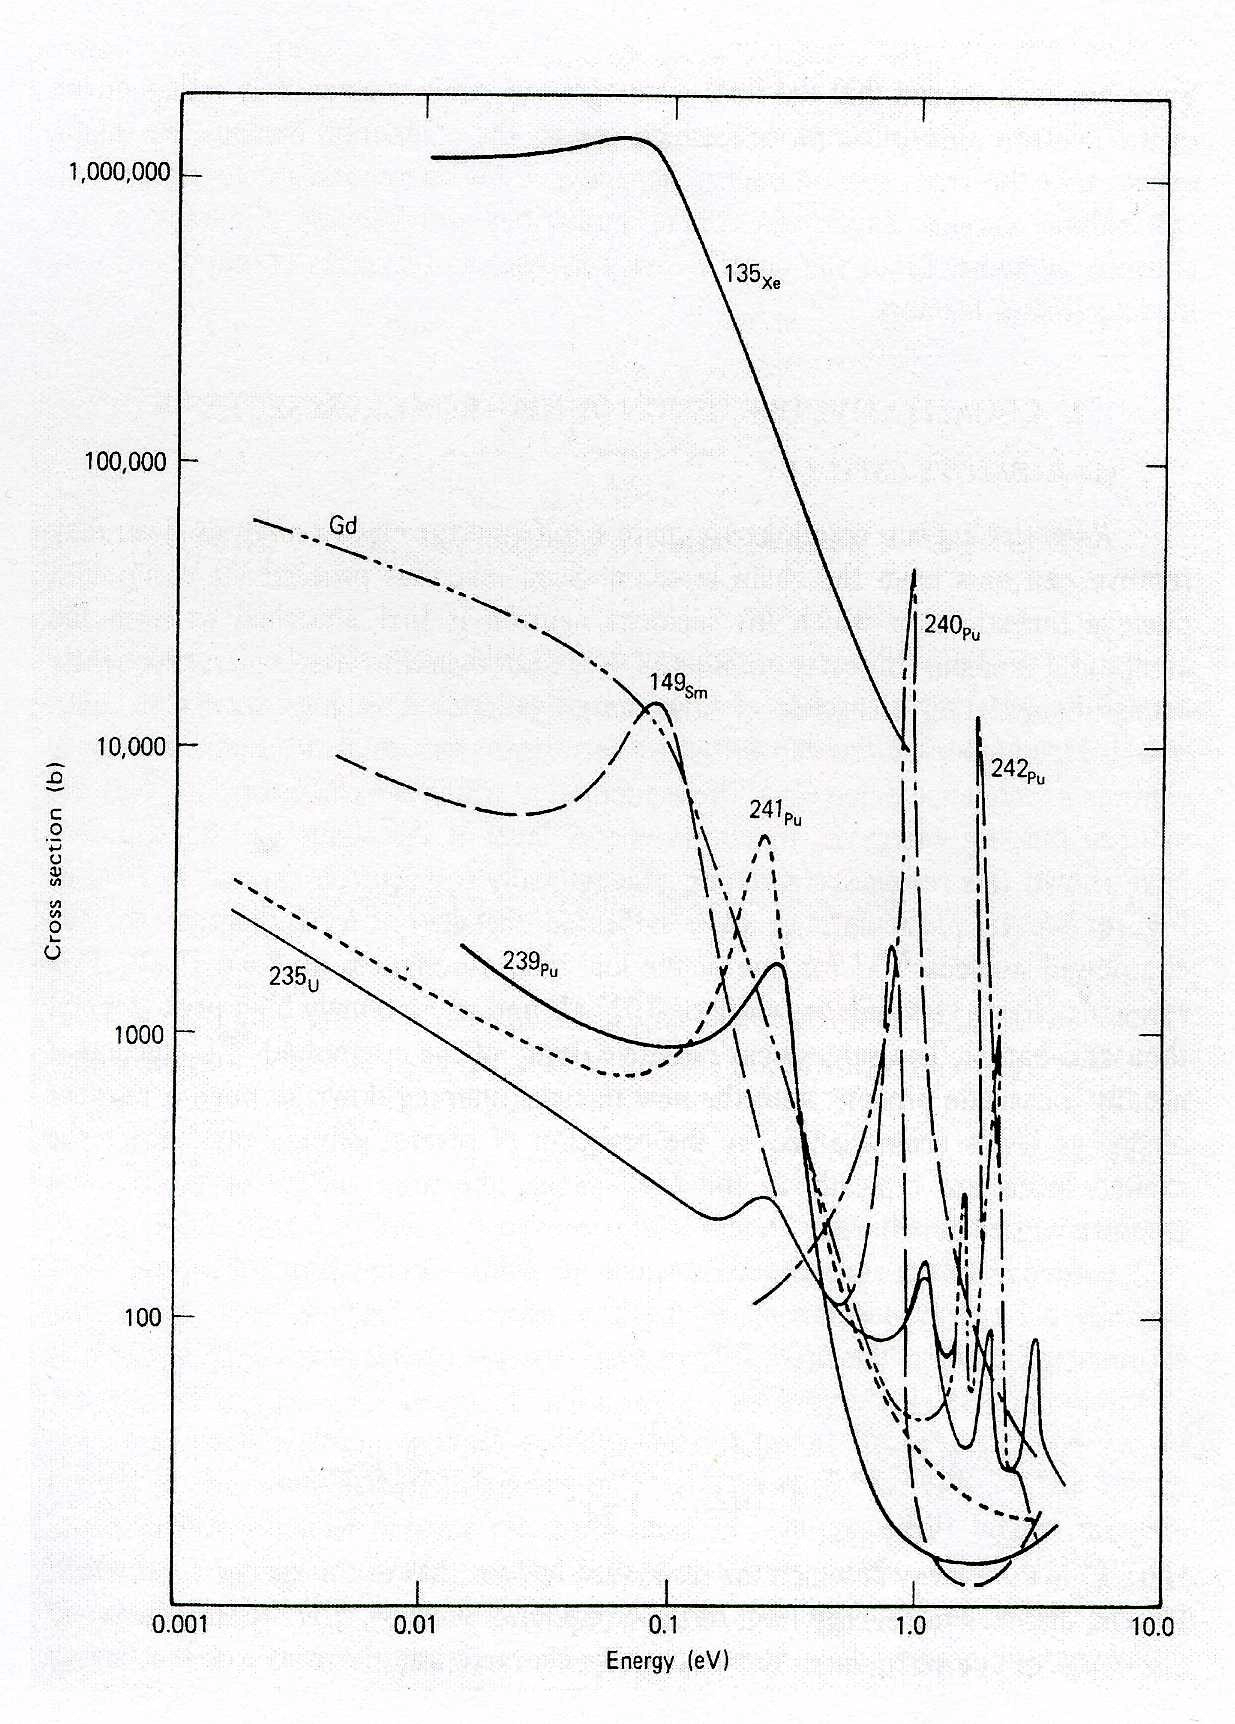
\includegraphics[scale=0.13]{ch1/image3.png}
	\captionof{figure}{ }
	\end{wrapfigure}
	
Le terme de section efficace vient d'une analogie avec une vision de physique classique des collisions entre particules.
Imaginons qu'on envoit un neutron dans une zone de surface totale S. Dans cette zone se trouvent des atomes
avec lesquels le neutron peut entrer en collision. En supposant qu'ils soient sphériques avec un rayon r, ils occupent
chacun une aire de $\pi r^2$ sur la zone. La probabilité que le neutron entre en collision avec un de ces atomes sera
donnée par le rapport la surface occupée par les atomes et de la surface totale : $\frac{n \pi r^2}{S}$ (n étant le
nombre d'atomes dans la surface). Le terme de section efficace vient donc du fait que la section efficace microscopique
\footnote{remarquer les unités $[cm^{2}]$} correspond à cette section transverse des atomes qui donnerait la même probabilité
d'interaction.\footnote{cf wikipédia si pas bien expliqué}\\

La section efficace\footnote{paragraphe pas très clair... Faut-il le garder ?} est ici la section transverse (attention, même expression pour les deux en 
anglais même lorsqu'elles ne sont pas égales). On peut voir une section efficace comme un disque 
de probabilité qui peut grandir ou diminuer en fonction de la probabilité d'avoir interaction. C'est 
une notion qui remplace quelque part la section transverse géométrique.\\

Historiquement, l'unité usuelle de la section efficace microscopique vient du fait qu'on imagine 
un neutron qui arrive face à une porte de grange (\textit{barn}) 
devant lui. On utilise alors cette unité plus adaptée : $1\ barn : 10^{-24}\ cm^2$.\\

La section efficace dépend de l'énergie comme on le verra par la suite.
Lorsqu'un neutron est libéré par une fission, il possède une énergie de l'ordre du MeV.
Il peut ensuite ralentir jusqu'à être en équilibre thermique avec le milieu, aux énergies dites 
"thermiques" \footnote{C'est bien les énergies de l'ordre de l'agitation du mouvement brownien ?} qui
sont de l'ordre de 0.025 eV. Il va donc falloir traiter des valeurs de l'énergies variant sur 8 ordres
de grandeur !\\

Le graphique de la section efficace en fonction de l'énergie est un peu chaotique. A une température 
équivalent d'$\frac{1}{40}eV$ on retrouve des pics (résonance) : on ne parle plus de capture, 
fission, \dots \ mais de section efficace totale.\\

Regardons la gamme d'énergie que l'on peut rencontrer sur un réacteur. Un neutron émis par 
fission a une énergie d'environ 2 MeV. Or, la probabilité de fission à cette énergie (donnée par
la section efficace) est plus petite de trois ordres de grandeur que la probabilité de fission
aux énergies thermiques. Si on souhaite avoir suffisamment de neutrons pour qu'il y ait assez de fissions,
 il peut être intéressant de ralentir les neutrons pour les amener dans la zone 
thermique "à gauche" afin d'avoir une section efficace de fission plus élevée.
Malheureusement, il faudra d'abord traverser la zone de résonance au milieu du graphe qui correspond
à des énergies pour lesquelles beaucoup de neutrons sont absorbés mais peu génèrent une fission.
\footnote{On pourrait demander plus de détails sur en quoi la résonance est si mauvaise ? La section
efficace de fission y est quand même élevée...}

\begin{center}
	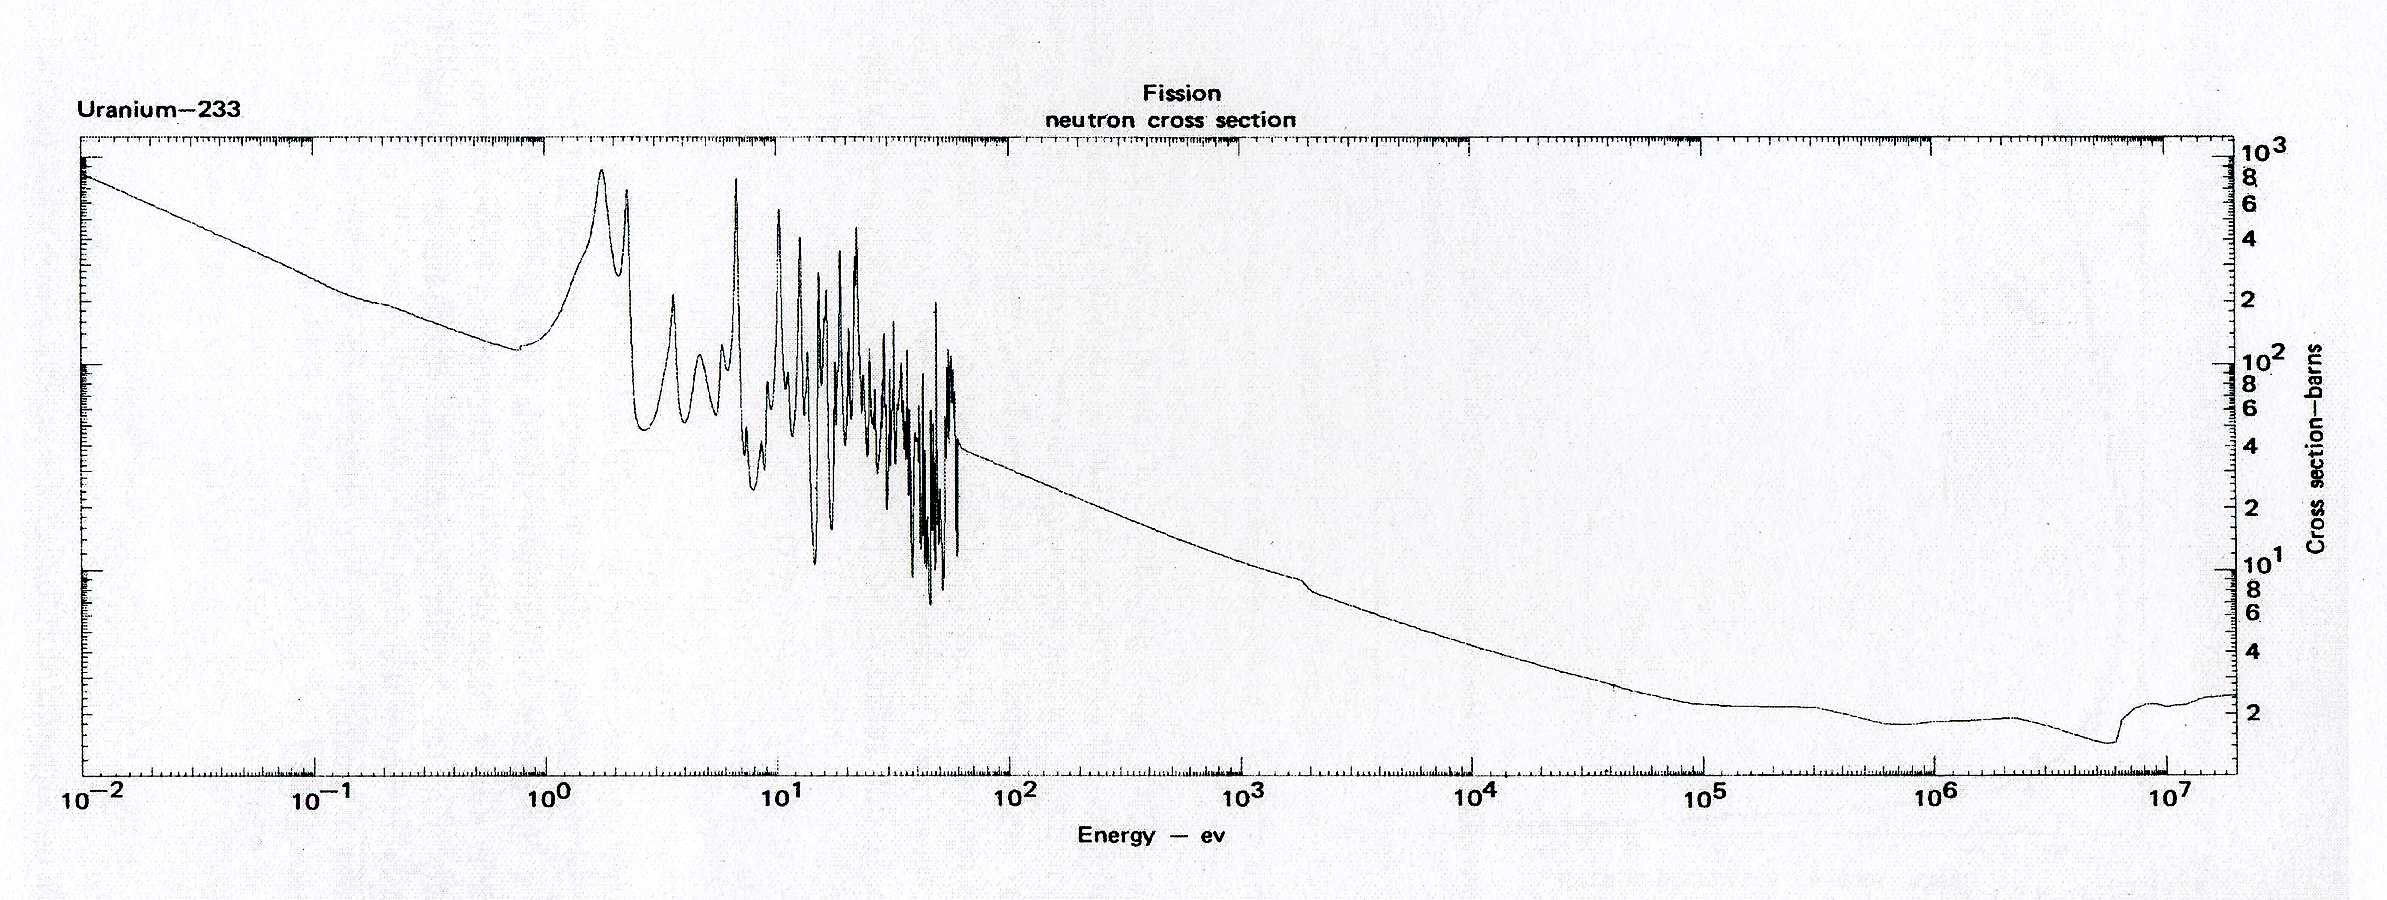
\includegraphics[scale=0.2]{ch1/image4.png}
	\captionof{figure}{ }
\end{center}


Pour ralentir les neutrons, il faudrait qu'ils entrent en collisions avec une autre particule, de masse semblable de sorte à avoir
un bon transert de l'énergie cinétique lors des chocs élastiques. Les protons ayant une masse proche de celle des neutrons,
on va utiliser l'eau pour jouer le rôle de ralentisseur de neutrons vers les énergies thermique, en plus de son rôle de fluide
caloporteur. Les neutrons ralentis jusqu'à atteindre une énergie thermique portent le nom de  \textit{neutrons thermiques}.
\newpage

\begin{center}
	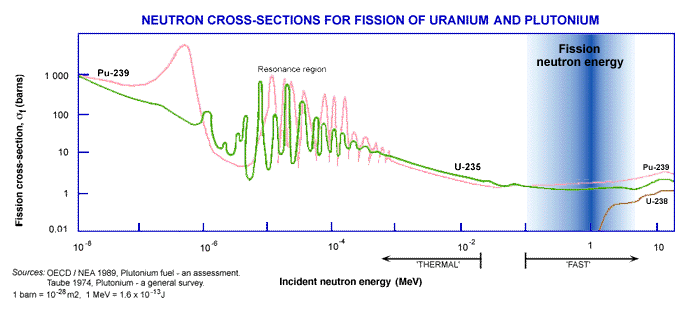
\includegraphics[scale=0.67]{ch1/image5.png}
	\captionof{figure}{ }
\end{center}

Il existe tout de même une petite marge pour tout de même faire autre chose : maintenir les énergies 
assez élevée afin de produire plus de matière fissile que ce qui a été consommé. En effet, si on 
parvient à légèrement monter les énergies il sera possible que l'$U_{238}$ produise par capture radiative
de la nouvelle matière fissile, le $Pu_{239}$ qui possède l'avantage d'émettre beaucoup de neutrons par fission.
On parle de \textit{neutrons rapides} lors de ce type d'utilisation.
Pour les accélérer il ne faut pas utiliser de l'eau mais des éléments lourds.
On définit le \textbf{breeding ratio}, $BR = \frac{taux\ de\ production\ de\ matière\ fissile}{taux\ de\ destruction\ de
matière\ fissile}$ afin d'avoir un critère pour le bon fonctionnement du réacteur rapide : $BR > 1$.



\subsection{Cycle neutronique et criticité}
\subsubsection{Caractéristique d'un cycle}
	\begin{wrapfigure}[7]{r}{4cm}
	\vspace{-5mm}
	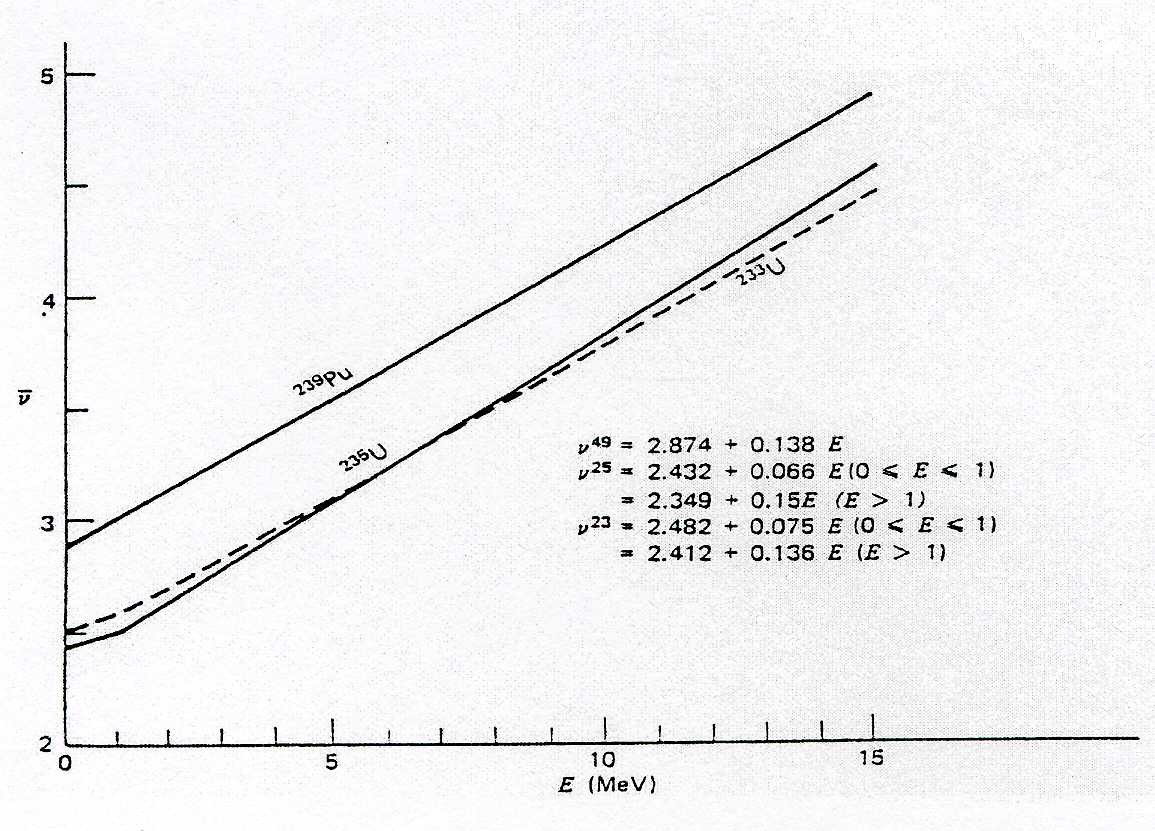
\includegraphics[scale=0.10]{ch1/image6.png}
	\captionof{figure}{ }
	\end{wrapfigure}
On souhaiterait avoir une réaction auto-entretenue. Pour se faire, on est en possession du nombre 
moyen de neutrons émis par fission. Pour l'$U_{235}$
\begin{equation}
\nu(E) = \left\{\begin{array}{ll}
2.432 +0.66E&\quad E\geq 1\\
2.349+0.15E&\quad E>1
\end{array}\right.
\end{equation}

\subsubsection{Paramètre de régénération}
Un autre paramètre souvent introduit est le paramètre de régénération $\eta$. La différence par rapport à $\nu$ est qu'il 
fait le bilan des neutrons qui ont été produits par rapport à ceux qui ont été consommés.
On exprime $\eta$ en multipliant le nombre de neutron moyen émis par
fission par la probabilité d'avoir une fission (donc la probabilité qu'un neutrons produit par 
fission donne lieu à une nouvelle fission) et l'on divise le tout par le nombre de neutrons
absorbés\footnote{L'absorption comprend à la fois la fission et la capture radiative.} : c'est le \textbf{paramètre de régénération}
\begin{equation}
\eta = \dfrac{\text{Nb $n$ produced in the fuel}}{\text{Nb $n$ absorbed in the fuel}}\quad\Rightarrow
\quad \eta = \dfrac{\nu\sigma_f}{\sigma_f+\sigma_c}=\dfrac{\nu}{1+\alpha}
\end{equation}
où $\alpha = \sigma_c/\sigma_f$. Ce paramètre dépend fortement de l'énergie. S'il y a plusieurs 
isotopes, il faut tenir compte des densités isotropiques (la section efficace macroscopique donne
le nombre moyen pondéré)
\begin{equation}
\eta = \dfrac{\sum_j\nu_j\Sigma_{fj}}{\sum_j \left(\Sigma_{fj}+\Sigma_{cj}\right)}
\end{equation}


\subsubsection{Breeding ratio (taux de reproduction)}
Ce ratio est lié au fait qu'il y a un excès de neutrons par rapport à ce qui est consommé : si l'on 
fait le bilan, on obtient chaque fois un nombre supplémentaire. Si $F$ est la fraction de ces 
neutrons qui vont être absorbés par le matériau fertile pour donner naissance à l'isotope associé, 
on définit le \textbf{breeding ratio} par
\begin{equation}
BR = (\eta-1)F
\end{equation}
où $\eta-1$ est l'excès de neutrons disponibles pour la reproduction.\\

\textsc{Criticité}\\
On parle de \textit{criticité} lorsque le réacteur peut fonctionner de façon stationnaire sans 
qu'il y ait apport extérieur de neutron : ce-dernier produit tous les neutrons nécessaires.
On a donc dans ce cas un neutron produit pour un neutron consommé en moyenne.
Cet équilibre 1/1 dépend d'une configuration générale du réacteur. Un réacteur critique est donc 
une condition d'équilibre qui n'a \textbf{rien à voir avec la puissance}.

\newpage
Afin de savoir si l'on est à la criticité, on introduit le facteur de multiplication du réacteur $k$ qui est 
le nombre moyen de neutrons émis lors d'un cycle complet par neutron envoyé initialement. 
On peut déterminer que l'on aura un réacteur sous-critique si k < 1, un réacteur critique si k = 1 et
un réacteur surcritique si k > 1.

Voyons comment exprimer ce facteur dans le cadre d'un réacteur infini\footnote{Le réacteur infini correspond
à un cas fictif permettant de simplifier les calculs}. \\

	\begin{wrapfigure}[14]{r}{10cm}
	\vspace{-5mm}
	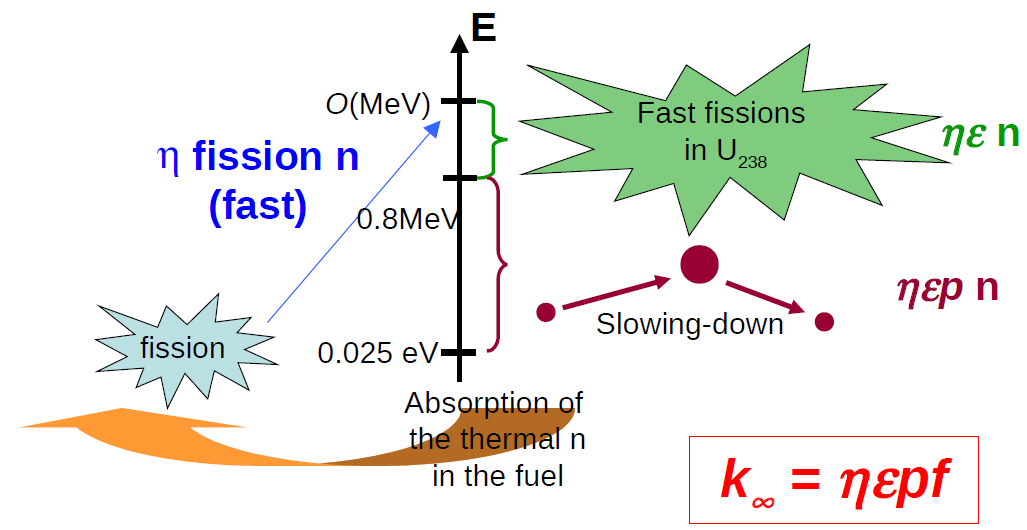
\includegraphics[scale=0.27]{ch1/image7.png}
	\captionof{figure}{ }
	\end{wrapfigure}
	
Partons d'un gentil petit neutron thermique (fraction d'eV) absorbé par le combustible. Combien 
de ces neutrons vont être émis ? C'est le fameux paramètre $\eta$. A partir d'un neutron, on a 
$\eta$ neutrons émis suite aux fissions. Une fraction de ces $\eta$ neutrons sont dans 
la gamme rapide et vont conduire à des fissions, augmentant le nombre de neutrons rapides d'un facteur $\epsilon$. Ces
neutrons vont ensuite ralentir et doivent survivre à ce ralentissement : seulement une fraction 
$p$ (probabilité anti-trappe ou probabilité d'échapper à la résonance) survit. On a donc pour un neutron $\eta\epsilon p$ qui atteignent 
le domaine thermique et $f$ (facteur d'usage thermique) d'entre-eux sont absorbés par le combustible et "recommencent" le cycle. 
On obtient la \textit{formule des quatre facteurs}
\begin{equation}
k_\infty = \eta\epsilon  pf
\end{equation}

Ceci est pour le cas d'infini, mais dans un cas réel il va y avoir des fuites : $P_f$ est la 
probabilité de ne pas sortir du réacteur lors du ralentissement et $P_{th}$ la probabilité de ne pas se sortir
du réacteur une fois aux énergies thermiques en attendant l'absorption\footnote{Il manque l'autre image qui est sur
même slide que image8}. 
\begin{equation}
k_{eff} = k_\infty P_fP_{th} = \eta \varepsilon pfP_fP_{th}
\end{equation}

	\begin{wrapfigure}[11]{l}{7.5cm}
	\vspace{-5mm}
	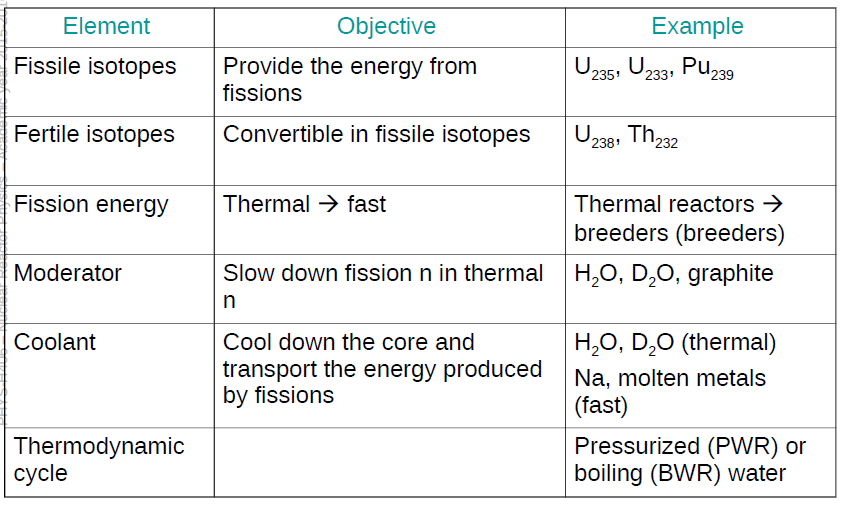
\includegraphics[scale=0.25]{ch1/image8.png}
	\captionof{figure}{ }
	\end{wrapfigure}
Comme $P_fP_{th} < 1$, il faut que $k_\infty > 1$ pour pouvoir atteindre la criticité. En pratique $1 \ll k_\infty$ car lorsque le 
réacteur tourne, il produit beaucoup de déchets. La capacité d'émettre des neutrons avec du 
combustible "frais" est plus importante en fin de cycle. Il peut donc y avoir un certain 
empoisonnement du réacteur. Tous ces facteurs $P,k_\infty$ dépendent de la géométrie et la 
nature des matériaux : il s'agit d'une balance entre la géométrie et les propriétés 
neutroniques\footnote{Si on souhaite faire monter la puissance d'un réacteur, il faut 
aller au delà de la criticité.}.\\


On a parle de survie aux fuites  mais un réacteur n'est pas dans un vide absolu. Quand un 
neutron quitte le réacteur on le reverra plus. Dans la réalité il serait pas mal d'utiliser 
un "réflecteur" : un matériau qui se trouve autour du combustible pour tenter de 
rétrodiffuser une partie de ces neutrons qui se font la maille. Ce n'est personne d'autre 
que l'eau qui joue ce rôle : l'eau a donc un rôle caloporteur, modérateur mais aussi réflecteur. \\

On définit la \textit{réactivité} comme la distance par rapport à la criticité. La protection 
majeure est l'utilisation de barres qui absorbe les neutrons. En cas d'arrêt d'urgence 
("\textit{scram}") ces barres sont plongées et le réacteur est au moins à l'arrêt malgré beaucoup de
chaleur émise par certaines réactions qui prendront du temps avant de disparaître.

\section{Profil de section efficaces}
\subsection{Mécanismes d'interactions}
Les longueurs d'onde $\lambda$ associées aux neutrons pour les énergies considérées sont bien 
supérieures à la taille des noyaux, ce qui permet de considérer une réaction du noyau dans son ensemble
et non pas pour chacun de ses nucléons. Deux mécanismes peuvent se produire :
\begin{enumerate}
\item Scattering de potentiel : choc sans interactions avec la structure interne du noyau
\item Résonances : interaction avec la structure interne (constitution d'un noyau 
composé puis désexcitation). L'énergie d'excitation dépendra de l'énergie de liaison du
noyau et de l'énergie cinétique associée au mouvement relatif entre le neutron et le noyau.
\end{enumerate}

\subsubsection{Énergie apportée par un neutron incident sur un noyau}
Considérons comme système de départ un neutron incident et un autre corps qui est un noyau $(A,Z)$.
L'énergie totale de ce système est donnée par la somme des énergies de masse du noyau et du neutron
et de l'énergie cinétique associée à leur mouvement relatif :
\begin{equation}
E_{tot} = m_{(A,Z)}c^2 + m_nc^2+E_{cin}
\end{equation}
Le second système est un noyau composé $(A+1, Z)$ issu de la collision.
\footnote{Pour le second système, l'énergie cinétique correspond au mouvement du noyau composé
par rapport à la position du noyau initiale ? Comment obtenir la valeur de cette nouvelle énergie cinétique ?
S'agit-il en fait de l'énergie cinétique du centre de masse ? Aussi pour le système 1 ?}
Le défaut de masse fait qu'on doit rajouter un terme pour que l'énergie totale soit conservée.
\begin{equation}
E_{tot}=E_{tot} = m_{(A+1,Z)}c^2 +E_{cin}+\dots\ ? 
\end{equation}
Il y a donc un manque au niveau de l'énergie totale. Faisons un bilan en calculant l'énergie 
associé au défaut de masse du noyau ($B$ pour \textit{bind}, lier).
On obtient l'énergie de liaison associée au défaut de masse comme la somme des énergies de 
masses des neutrons et des protons à laquelle on soustrait l'énergie de masse du noyau formé :
\begin{equation}
B(A,Z) = (A-Z)m_nc^2+Zm_pc^2 - m_{(A,Z)}c^2
\end{equation}
L'énergie à fournir au système pour séparer un neutron du noyau $(A+1,Z)$ s'obtient en soustrayant l'énergie de liaison
du nouveau noyau à l'énergie du noyau initial (on doit vaincre la liaison initiale mais on est aidé par la liaison finale) :
\begin{equation}
S_n = B(A+1,Z)-B(A,Z) = m_nc^2+m_{(A,Z)}c^2-m_{(A+1,Z)}c^2
\end{equation}
C'est précisément ce qu'il nous manquait pour avoir conservation de l'énergie : il faut 
rajouter l'énergie de séparation.
\begin{equation}
E_{tot}=E_{tot} = m_{(A+1,Z)}c^2 +E_{cin}+S_n
\end{equation}

	\begin{wrapfigure}[10]{l}{7.5cm}
	\vspace{-8mm}
	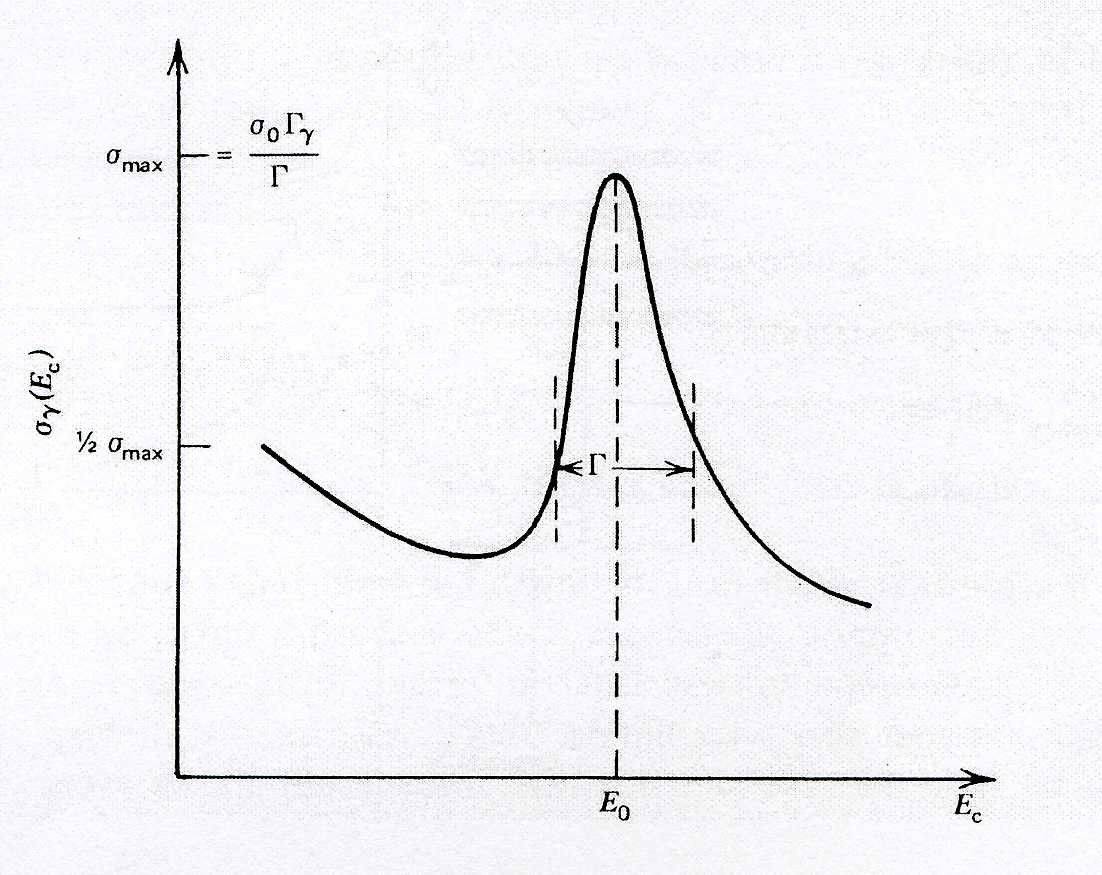
\includegraphics[scale=0.17]{ch1/image9.png}
	\captionof{figure}{ }
	\end{wrapfigure}
	
On peut voir cette "énergie de séparation" comme l'énergie qu'apporte "en plus" de son énergie 
cinétique un neutron\footnote{Euh l'énergie de séparation n'est pas liée au défaut de masse du noyau plutôt ?
Pourquoi ce serait le neutron incident qui l'apporte ? Ou est-ce que tu veux dire que dans le premier
système le neutron apporte une énergie $E_{cin}+S_n$ et pas juste $E_{cin}$ pour qu'il y ait fission ?
Il faudrait clarifier, c'est un peu confus.}.	
C'est une caractéristique non banale car on peut interpréter cette variation 
du défaut de masse comme le fait qu'une particule apporte en plus que son énergie cinétique une 
énergie un peu plus importante que la réalité du fondamental. 

\subsection{Sections efficaces associées}
\subsubsection{Capture radiative $\gamma$}
Il s'agit du modèle typique : un neutron est absorbé, il forme un noyau composé qui se 
désexcite en se réorganisant vers un état plus stable, ce qui s'accompagne de l'émission d'un photon
\begin{center}
neutron absorbé $\longrightarrow$ noyau composé $\longrightarrow$ $\gamma$
\end{center}
On sait que la section efficace microscopique de capture radiative doit présenter une résonance
aux niveaux d'énergies $E$ du noyau composé. La distribution de Breit-Wigner permet de modéliser cette dépendance
\begin{equation}
{\sigma _\gamma } = \frac{\pi }{{{k^2}}}{g_J}\frac{{{\Gamma _n}{\Gamma _\gamma }}}{{{{(E - {E_o})}^2} + {\textstyle{{{\Gamma ^2}} \over 4}}}} \equiv {\sigma _o}\frac{{{\Gamma _\gamma }}}{\Gamma }\frac{1}{{1 + {x^2}}}
\end{equation}
où k est le nombre d'onde ($k^2$ est donc proportionnel à l'énergie), $g_j$ est le facteur de spin statistique,
$\Gamma_\gamma$, $\Gamma_n$ et $\Gamma = \Gamma_\gamma + \Gamma_n$ sont les largeurs des pics (de capture, de scattering
et total) et  $x= \frac{E-E_0}{\gamma/2}$. On retrouve les largeur de raie $\gamma$ et un comportement en 
l'inverse de l'écart entre deux résonance. On peut même obtenir un comportement en $1/(1+x^2)$ si 
on utilise l'énergie \textit{relative} de la demi-largeur de raie. On peut voir ci-contre que 
en dehors des pics, on retrouve une gentille décroissance hyperbolique. Plus l'énergie est élevée, 
plus on observe une décroissance.

\subsubsection{Scattering (diffusion)}
\textsc{Diffusion élastique}\\
\textbf{Scattering de potentiel}

Le scattering de potentiel correspond aux cas où le neutron est dévié de sa trajectoire par le noyau
d'une manière similaire à la vision de la physique classique tout en conservant l'énergie cinétique
du centre de masse. Ce processus ne se produit que si l'énergie du neutron n'est pas trop élevée.
On associera au scattering de potentiel une section efficace microscopique valable dans l'intervalle
d'énergie [1eV, 1MeV] :
\begin{equation}
\sigma_{pa} = 4 pi R^2
\end{equation}
où l'on retrouve le rayon du noyau R et où le facteur 4 vient d'un effet quantique.\\

\textbf{Résonance de la diffusion élastique}

Dans ce cas, le neutron est absorbé puis réémis avec une autre direction tout en conservant
l'énergie cinétique du centre de masse du système.
(c'est dans le mouvement relatif entre le neutron et le noyau que l'énergie est conservée)
\footnote{Que veux-tu dire exactement dans cette parenthèse ?}
\begin{center}
neutron absorbé $\longrightarrow$ noyau composé $\longrightarrow$ neutron réémis à "la même" énergie
\end{center}


On modélise la section efficace microscopique de scattering $\sigma_s$ en tenant compte
de la résonance dans le phénomène de capture, du scattering de potentiel et d'une interférence :
\begin{equation}
{\sigma _s} = \frac{\pi }{{{k^2}}}{g_J}\frac{{{\Gamma _n}{\Gamma _\gamma }}}{{{{(E - {E_o})}^2} + {\textstyle{{{\Gamma ^2}} \over 4}}}} + \frac{{4\pi R}}{k}{g_J}\frac{{{\Gamma _n}(E - {E_o})}}{{{{(E - {E_o})}^2} + {\textstyle{{{\Gamma ^2}} \over 4}}}} + 4\pi {R^2}
\end{equation}
Le premier terme est une lorentzienne près du pic de résonance et un terme supplémentaire lié aux 
interférences. Le comportement en énergie est différent et il est important de s'en souvenir. \\

\textsc{Diffusion inélastique}\\
Lors de la diffusion inélastique, l'énergie cinétique du centre de masse n'est pas conservée.
Le neutron est absorbé par le noyau pour former un noyau composé. Celui-ci se réorganise et
se désexcite en réémettant le neutron ainsi qu'un photon $\gamma$.
Ici, la perte d'énergie est compensée par l'émission d'un photon gamma (lors de la désexcitation 
du noyau)
\begin{center}
neutron absorbé $\longrightarrow$ noyau composé $\longrightarrow$ neutron réémis à $E<E_i$
et désexcitation du noyau par émission $\gamma$
\end{center}
La probabilité de diffusion inélastique est nulle jusqu'à un certain seuil car il faut que le neutron
ait assez d'énergie que pour exciter le premier niveau du noyau ($\approx 10\ keV$ pour les 
noyaux lourds, plus élevé pour les noyaux légers)\footnote{Voir note, qqch pas clair avec la 
raison pour laquelle l'inélastique convient pas.}. 
Le seuil d'énergie étant beaucoup plus grand pour les noyaux légers, on peut suposer qu'il n'y
a presque pas de diffusion inélastique à l'intérieur d'un réacteur nucléaire.
%Comme l'énergie est trop faible, ce type de diffusion n'aura que des effets dont nous ne tiendrons pas compte. 
%Il faut garder à l'esprit que l'on peut ralentir le neutron sens perte d'énergie car c'est le 
%mouvement relatif entre noyau et neutron qui est la caractéristique du scattering : on les modère élastiquement.
La thermalisation des neutrons se fera donc presque exclusivement par diffusion élastique : il faut garder
à l'esprit que c'est l'énergie cinétique du neutron dans le référentiel du noyau qui est conservée dans ce
cas, ce qui veut dire que ce type de diffusion peut ralentir les neutrons dans le référentiel du réacteur.\\

\textsc{Fission}\\
Nous utiliserons un modèle simple :
\begin{center}
neutron absorbé $\longrightarrow$ noyau composé $\longrightarrow$ neutrons réémis \dots
\end{center}
\dots + une désexcitation du noyau par fragmentaton en deux (ou trois) noyaux plus léger. Il 
peut exister un seuil d'énergie pour déclencher la fission. S'il n'y a pas de seuil, le noyau
sera fissile.




\newpage
\section{Fission nucléaire}
\subsection{Description}
Essayons de retrouver les éléments qui constituent ce phénomène de fission. Séparons l'énergie de 
séparation d'un neutron
\begin{equation}
{S_n} = B(A,Z) - B(A - 1,Z)  {\kern 1pt} {\kern 1pt}  = \frac{{B(A,Z)}}{A} + (A - 1).
\underbrace{\left( {\frac{{B(A,Z)}}{A} - \frac{{B(A - 1,Z)}}{{A - 1}}} \right)}_{<0}
\end{equation}
L'énergie $S_n$ est inférieure à l'énergie de liaison moyenne $E$ par nucléon pour un noyau lourd.
$S_n$ est l'énergie minimale qu'il faut fournir pour passer d'un noyau $(A-1,Z)$ à un noyau composé $(A,Z)$.

\subsubsection{Formule semi-empirique  pour la masse d'un noyau}
En première approximation, l'énergie de liaison est proportionnel au nombre de masse. Ceci implique 
que 
$$m(\text{noyau}) \propto A$$
Le rayon d'un noyau est donné par $R=r_0.\sqrt[3]{A}$ impliquant que
$$V(\text{noyau}) \propto A$$
En supposant une densité +/- constante et que le noyau se comporte comme un liquide incompressible, 
on peut utiliser la formule semi-empirique de Weizsäcker
\begin{equation}
B(A,Z) = {a_v}A - {a_s}{A^{2/3}} - {a_a}\frac{{{{(A - 2Z)}^2}}}{A} - {a_c}\frac{{{Z^2}}}{{{A^{1/3}}}} + \delta (A,Z)
\end{equation}
où les deux premiers termes sont dus à la tension superficielle, le troisième à l'asymétrie $N-Z$, le quatrième
à la répulsion coulombienne et le dernier est un facteur de parité de spin : ce terme est dominant 
pour les noyaux lourds
\begin{equation}
\delta(A,Z) = \left\{\begin{array}{ll}
\frac{a_p}{A^{3/4}} & Z, N\ \text{pairs}\\
0 & A\ \text{impair}\\
-\frac{a_p}{A^{3/4}} & Z, N\ \text{impairs}
\end{array}\right.
\end{equation}
Dans un cas l'énergie de liaison augmente à cause du spin et dans l'autre pas
\begin{enumerate}
\item Noyau (Z pair, N impair) $\to$ Noyau (Z pair, N pair) $\Rightarrow +a_p/A^{3/4}$
\item Noyau (Z pair, N pair) $\to$ Noyau (Z pair, N impair) $\Rightarrow -a_p/A^{3/4}$
\end{enumerate}
Il\footnote{S'assurer qu'on a bien compris ce paragraphe...}
 en résulte une différence de $S_n = 2a_p/A^{3/4}$ soit de l'ordre du MeV! On voit donc 
que si on fissioner avec un neutron thermique dans le second cas, il faut lui adjoindre une énergie cinétique 
supplémentaire de quasi 1 MeV pour compenser cette énergie\footnote{C'est le seuil d'énergie à fournir 
pour rendre un matériau fertile fissile.}. 



\subsubsection{Fission spontanée v.s. induite}
\subsubsection{Capture $\gamma$}
	\begin{wrapfigure}[14]{l}{7.5cm}
%	\vspace{-5mm}
	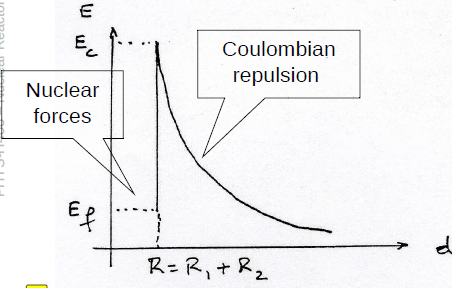
\includegraphics[scale=0.475]{ch1/image10.png}
	\captionof{figure}{ }
	\end{wrapfigure}
Soit une réaction de fission
\begin{equation}
(A,Z) \to (A_1,Z_1)+(A_2,Z_2)
\end{equation}
La masse du noyau initial est supérieur à celle des fragments.\footnote{D'où on sort ça ? C'est pas en contradiction
avec le défaut de masse ?} Est-il possible de voir un tel 
phénomène apparaître de façon spontanée ? Oui, mais pas observée. L'énergie potentielle des 
fragments est une fonction de la distance entre eux :$E_c$ l'énergie du potentiel de Coulomb, $d
=R_1+R_2$ la distance entre les charges $Z_1,Z_2$, $E_f$ la différence d'énergie de liaison entre 
$(A,Z)$ et ses fragments. Les noyaux sont "un peu" trop gros pour l'effet tunnel. \\

	\begin{wrapfigure}[14]{r}{7.5cm}
	\vspace{-5mm}
	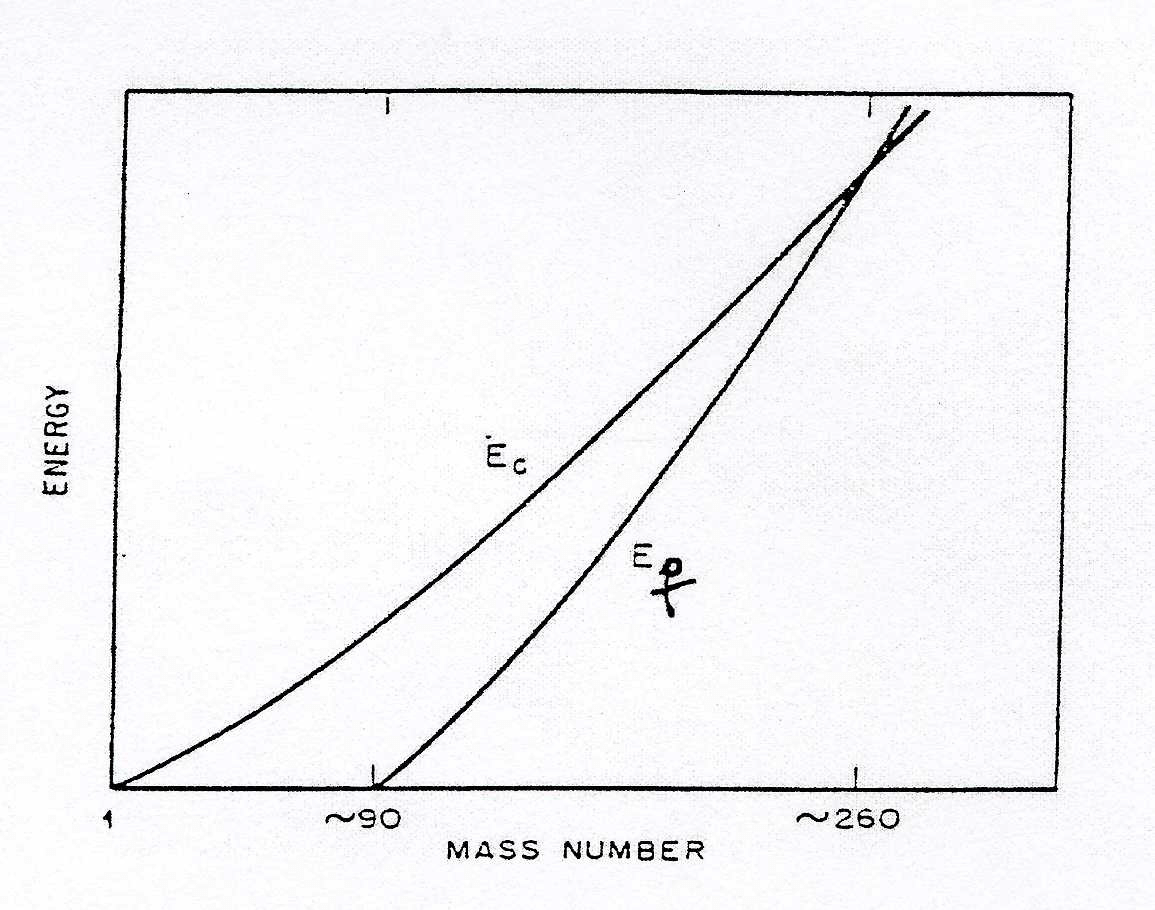
\includegraphics[scale=0.2]{ch1/image11.png}
	\captionof{figure}{ }
	\end{wrapfigure}
L'énergie permettant la fission est apportée par le neutron ($S_n+E_{cin}$) pour compenser 
$E_c-E_f$ (différence d'énergie entre coulomb et fission). Prenons par exemple la fission 
symétrique. Des que l'on dépasse 260 comme nombre de masse, on n'a plus de noyau stable. Dans 
l'intervalle qui nous intéresse $A\in[230,240]$, la différence entre la hauteur de la barrière 
coulombienne et le fond du puits est de l'ordre de $E_c-E_f=6$ MeV et l'énergie de liaison amenée par 
le neutron est du même ordre de grandeur $S_n = 6$ MeV. Avec cette énergie apportée on est à 
la hauteur de la barrière à franchir, il suffit d'un petit surplus d'énergie qui est apporté 
par l'énergie cinétique : la fission induite est possible.
\footnote{Quid de la première divergence ?}\\


\subsubsection{Développement d'une fission induite (capture $(n,f)$)}
Le temps d'un processus d'absorption est plus petit que $10^{-17}s$ alors que le temps de vie d'un 
noyau excité est de $10^{-14}$s ce qui est court, mais long par rapport au temps 
d'absorption d'un neutron : le système "a le temps d'oublier" les caractéristiques du neutron 
incident. Il n'y a donc pas de raison d'avoir une distribution anisotrope, toutes les directions 
d'émission sont équiprobables.\\

Par agitation des nucléons dans le noyau excité il se forme deux noyaux qui se font éjecter par 
la répulsion coulombienne dont la durée d'interaction est d'environ $10^{-20}$s. Comme on casse un noyau lourd, ces fragments ont un 
excédent de neutrons et sont hors équilibres. Pour se stabiliser, ils émettent directement 
($10^{-17}$s) des neutrons dit \textbf{prompts} : spectre isotrope donné par la distribution de Maxwell
\footnote{Il s'agit d'une distribution, elle aura donc les dimensions inverses de celle de sa variable.}
\begin{equation}
\chi (E) = \frac{2}{\theta }\sqrt {\frac{E}{{\pi \theta }}} .{e^{ - \frac{E}{\theta }}}
\end{equation}

Malgré ces émissions de neutrons, les fragments ne sont pas totalement désexcité et émettent 
des $\gamma$ (prompt, $10^{-14}s$) sur des temps courts.
Une grande partie de l'énergie libérée par la fission se trouve convertie en énergie cinétique
des fragments. Ceux-ci la perdront en partie par ionisation et excitation des atomes du milieu
croisé. Ces fragments étant des produits de fission, il sont instables et donneront lieu à des
désintégrations $\beta$.
% L'énergie cinétique des fragments 
%reprend une grande partie des 200 MeV disponibles. Ces fragments, produits de fissions, sont 
%parti pour des désintégrations $\beta$ car déficit de protons présent.


\subsection{Neutrons retardés}
Les produits de fission impliqués dans les chaînes radioactives sont en général dans un
état excité. La désexcitation se fait souvent par émission d'un photon $\gamma$ mais il
arrive quelque fois qu'elle soit accompagnée de l'émission d'un neutron si l'énergie
d'excitation est suffisamment grande.
Le temps d'émission d'un neutron est lié au temps de demi-vie de l'isotope précédent
ce qui fait que ces neutrons sont émis beaucoup plus tardivement que les neutrons prompts :
on parle alors de \textbf{neutrons retardés}.
Les sources de neutrons retardés sont appelés les précurseurs.\\

Il existe au moins une cinquantaine de précurseurs que l'on regroupera en six classes, chacune
caractérisée par : un temps de demi-vie du précurseur $T_i$, une fraction $\beta_i$ de neutrons
de fission dans le groupe i, une énergie moyenne $E_i$ ainsi qu'un spectre $\chi_i(E)$.
De plus, nous ferons l'hypothèse que les précurseurs sont émis directement après la fission.

\subsubsection{Évolution de la population de neutrons $N$}
Soit $N$ le nombre de neutrons et $l$ la durée moyenne d'un cycle qui vaut $\approx 10^{-4}$s
\begin{equation}
\frac{dN}{dt} = \dfrac{k_{eff}-1}{l}N\quad\Leftrightarrow\quad N(t)=N(0)e^{\frac{k_{eff}-1}{l}t}
\end{equation}
Pour $N$ neutrons présent par cycle, on produit $k_{eff}-1$(1= celui que l'on a envoyé) neutrons.
Si $k_{eff}=1.001$ on trouve
\begin{equation}
\frac{N(1s)}{N(0)} \approx e^{10}\ !!!
\end{equation}
Ceci montre que dans ces conditions, toute modification du facteur de multiplication, même
mineure mène a une augmentation démesurée de la population neutronique !
Heureusement, la réalité est différentes car les temps caractéristiques sont beaucoup plus long 
grâce aux neutrons retardés\footnote{On a joute au $(1-\beta)l\approx 10^{-4}$ les temps de vie 
des neutrons retardés}
\begin{equation}
l \longrightarrow (1-\beta)l + \sum_i\beta_iT_i \approx 10^{-1}\ s
\end{equation}
Si $k_{eff}=1.001$ on trouve
\begin{equation}
\frac{N(1s)}{N(0)} \approx e^{0.01}
\end{equation}
Cette variation est tout à fait gérable. En conclusion, l'émission de neutrons retardés par les
précurseurs n'est peut-être que de 0.68\% mais c'est la clef pour le contrôle du réacteur car 
sans eux il ne serait pas possible d'intervenir sur la réaction pour la contrôler.
%il n'y a rien qui peut s'opposer à une variation de l'ordre de $e^{10}$.